\section{Date: 2026-09-15}
\noindent \textbf{Series ID: ATNHPIUS42020Q} 

\noindent This series is titled All-Transactions House Price Index for San Luis Obispo-Paso Robles, CA (MSA) and has a frequency of Quarterly. The units are Index 1995:Q1=100 and the seasonal adjustment is Not Seasonally Adjusted.The observation start date is 1977-10-01 and the observation end date is 2026-04-01.The popularity of this series is 8. \\ 

\noindent \textbf{Series ID: EARPRXDBNQ} 

\noindent This series is titled Percent of Value of Loans Prime Based by Average Loan Size (\$ thousands), Prime, Domestic Banks (DISCONTINUED) and has a frequency of Quarterly, 2nd Month's 1st Full Week. The units are Percent and the seasonal adjustment is Not Seasonally Adjusted.The observation start date is 1997-04-01 and the observation end date is 2017-04-01.The popularity of this series is 1. \\ 

\subsection{Raw Regression}
\noindent Regresses the two series against each other directly. A significant result here can come just as easily from both series sharing a long-run trend as from any real relationship.

\begin{center}
\begin{tabular}{lclc}
\toprule
\textbf{Dep. Variable:}              & value\_fred\_EARPRXDBNQ & \textbf{  R-squared:         } &     0.039   \\
\textbf{Model:}                      &           OLS           & \textbf{  Adj. R-squared:    } &     0.027   \\
\textbf{Method:}                     &      Least Squares      & \textbf{  F-statistic:       } &     3.241   \\
\textbf{Date:}                       &     Tue, 15 Sep 2026    & \textbf{  Prob (F-statistic):} &   0.0756    \\
\textbf{Time:}                       &         15:46:24        & \textbf{  Log-Likelihood:    } &   -364.17   \\
\textbf{No. Observations:}           &              81         & \textbf{  AIC:               } &     732.3   \\
\textbf{Df Residuals:}               &              79         & \textbf{  BIC:               } &     737.1   \\
\textbf{Df Model:}                   &               1         & \textbf{                     } &             \\
\textbf{Covariance Type:}            &        nonrobust        & \textbf{                     } &             \\
\bottomrule
\end{tabular}
\begin{tabular}{lcccccc}
                                     & \textbf{coef} & \textbf{std err} & \textbf{t} & \textbf{P$> |$t$|$} & \textbf{[0.025} & \textbf{0.975]}  \\
\midrule
\textbf{const}                       &     176.5714  &        8.976     &    19.671  &         0.000        &      158.704    &      194.438     \\
\textbf{value\_fred\_ATNHPIUS42020Q} &       0.0686  &        0.038     &     1.800  &         0.076        &       -0.007    &        0.144     \\
\bottomrule
\end{tabular}
\begin{tabular}{lclc}
\textbf{Omnibus:}       &  0.239 & \textbf{  Durbin-Watson:     } &    1.271  \\
\textbf{Prob(Omnibus):} &  0.887 & \textbf{  Jarque-Bera (JB):  } &    0.081  \\
\textbf{Skew:}          & -0.077 & \textbf{  Prob(JB):          } &    0.960  \\
\textbf{Kurtosis:}      &  3.017 & \textbf{  Cond. No.          } &     866.  \\
\bottomrule
\end{tabular}
%\caption{OLS Regression Results}
\end{center}

Notes: \newline
 [1] Standard Errors assume that the covariance matrix of the errors is correctly specified.

\begin{figure}
\centering
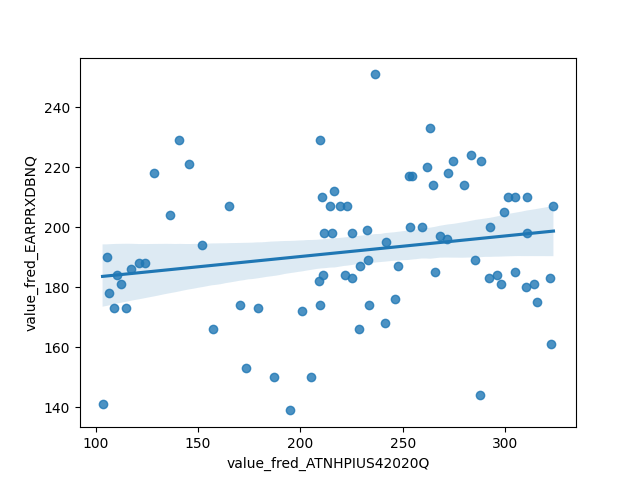
\includegraphics[scale = 0.9]{plots/plot_2026-09-15.png}
\caption{Raw Regression Plot for 2026-09-15}
\end{figure}
\newpage
\subsection{Detrended Regression}
\noindent Regresses the residuals of each series after removing its own linear time trend, so a shared trend can no longer drive the result on its own. A relationship that stays significant here is better evidence of a genuine link between the two series.

\begin{center}
\begin{tabular}{lclc}
\toprule
\textbf{Dep. Variable:}                         & value\_fred\_EARPRXDBNQ\_detrended & \textbf{  R-squared:         } &     0.027   \\
\textbf{Model:}                                 &                OLS                 & \textbf{  Adj. R-squared:    } &     0.015   \\
\textbf{Method:}                                &           Least Squares            & \textbf{  F-statistic:       } &     2.188   \\
\textbf{Date:}                                  &          Tue, 15 Sep 2026          & \textbf{  Prob (F-statistic):} &    0.143    \\
\textbf{Time:}                                  &              15:46:25              & \textbf{  Log-Likelihood:    } &   -356.02   \\
\textbf{No. Observations:}                      &                   81               & \textbf{  AIC:               } &     716.0   \\
\textbf{Df Residuals:}                          &                   79               & \textbf{  BIC:               } &     720.8   \\
\textbf{Df Model:}                              &                    1               & \textbf{                     } &             \\
\textbf{Covariance Type:}                       &             nonrobust              & \textbf{                     } &             \\
\bottomrule
\end{tabular}
\begin{tabular}{lcccccc}
                                                & \textbf{coef} & \textbf{std err} & \textbf{t} & \textbf{P$> |$t$|$} & \textbf{[0.025} & \textbf{0.975]}  \\
\midrule
\textbf{const}                                  &   -4.581e-12  &        2.207     & -2.08e-12  &         1.000        &       -4.393    &        4.393     \\
\textbf{value\_fred\_ATNHPIUS42020Q\_detrended} &      -0.0708  &        0.048     &    -1.479  &         0.143        &       -0.166    &        0.024     \\
\bottomrule
\end{tabular}
\begin{tabular}{lclc}
\textbf{Omnibus:}       &  1.694 & \textbf{  Durbin-Watson:     } &    1.556  \\
\textbf{Prob(Omnibus):} &  0.429 & \textbf{  Jarque-Bera (JB):  } &    1.096  \\
\textbf{Skew:}          &  0.241 & \textbf{  Prob(JB):          } &    0.578  \\
\textbf{Kurtosis:}      &  3.303 & \textbf{  Cond. No.          } &     46.1  \\
\bottomrule
\end{tabular}
%\caption{OLS Regression Results}
\end{center}

Notes: \newline
 [1] Standard Errors assume that the covariance matrix of the errors is correctly specified.

\begin{figure}
\centering
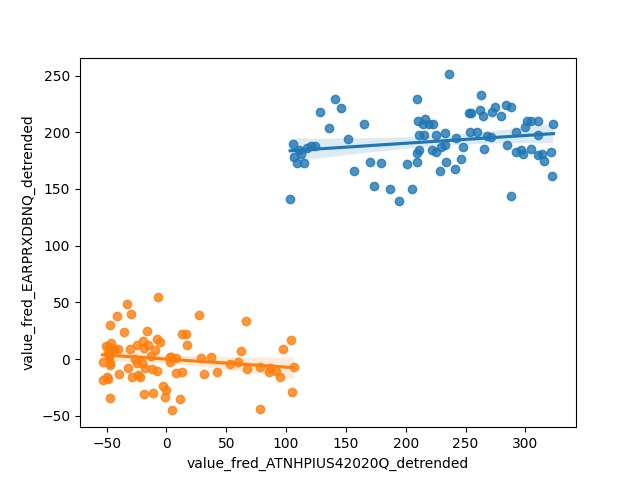
\includegraphics[scale = 0.9]{plots/plot_2026-09-15_detrended.png}
\caption{Detrended Regression Plot for 2026-09-15}
\end{figure}
\newpage
